\begin{figure*}[t!]
    \centering
    \begin{minipage}{0.48\linewidth}
        \centering
        \scriptsize
        \setlength{\tabcolsep}{2.9pt}
        \renewcommand{\arraystretch}{1.25} 
        \captionof{table}{\textbf{Quantitative results of quantity-aware image generation in NFE scaling expriment.} We use the same $100$ prompts from T2I-CompBench~\cite{Huang:2025T2ICompBench++}. \textsuperscript{\textdagger} denotes the given reward.}
        \label{tab:appendx_counting_nfe}
        \newcolumntype{Z}{>{\centering\arraybackslash}m{0.01\textwidth}}
        \newcolumntype{Y}{>{\centering\arraybackslash}m{0.2\textwidth}}
        \newcolumntype{W}{>{\centering\arraybackslash}m{0.15\textwidth}}
        \newcolumntype{X}{>{\centering\arraybackslash}m{0.11\textwidth}}
        \begin{tabular}{Z X | W W Y Y}
            \toprule
            & NFEs & \makecell{RSS\textsuperscript{\textdagger}\\\cite{Liu:2024GroundingDINO} $\downarrow$} & Acc. $\uparrow$ & \makecell{VQAScore~\cite{Lin:2024CLIPFlanT5}\\(held-out) $\uparrow$ } & \makecell{Aesthetic\\Score~\cite{Schuhmann:aesthetics} $\uparrow$} \\
            \midrule
            \multirow{5}{*}{\rotatebox{90}{BoN}} & 50 & 4.360 & 0.400  & 0.758  & 5.408 \\
            & 100 & 3.280 & 0.510  & 0.750  & 5.522 \\
            & 300 & 2.190 & 0.570  & 0.755  & 5.463 \\
            & 500 & 1.760 & 0.580  & 0.756  & 5.420 \\
            & 1000 & 1.340 & 0.590  & 0.759  & 5.466 \\
            \midrule
            \multirow{5}{*}{\rotatebox{90}{{\Oursbf{}} (Ours)}} & 50 & 3.250 & 0.410  & 0.756  & 5.560 \\
            & 100 & 1.860 & 0.590  & 0.760  & 5.627 \\
            & 300 & 0.690 & 0.720  & 0.779  & 5.503 \\
            & 500 & 0.540 & 0.800  & 0.769  & 5.581 \\
            & 1000 & 0.290 & 0.880  & 0.777  & 5.526 \\
            \bottomrule
        \end{tabular}
    \end{minipage}
    \hfill
    \begin{minipage}{0.48\linewidth}
        \centering
        {\scriptsize
        \setlength{\tabcolsep}{0.0em}
        \def\arraystretch{0.0}
        \newcolumntype{Z}{>{\centering\arraybackslash}m{\linewidth}}
        \begin{tabularx}{\linewidth}{Z}
            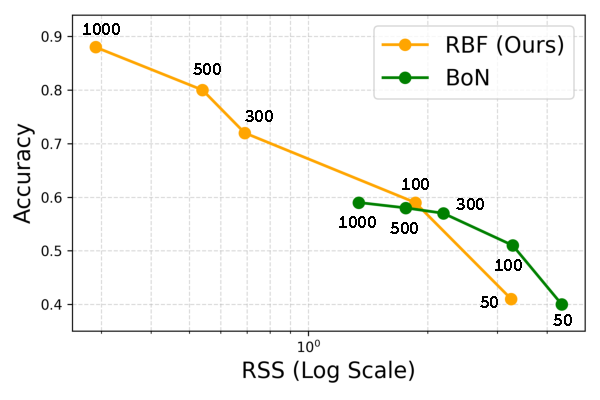
\includegraphics[width=\linewidth]{Figures/scaling/quantity_nfe_scaling.pdf}
        \end{tabularx}
        }
        \caption{
        \textbf{Quantity-aware image generation scaling behavior comparison of BoN and \Ours{}.} 
        We plot the known reward (RSS)~\cite{Liu:2024GroundingDINO} against accuracy for different numbers of function evaluations: $\{ 50, 100, 300, 500, 1,000 \}$. 
        Note that the horizontal axis is displayed on a logarithmic scale. 
        }
        \label{fig:appendix_nfe_scaling}
    \end{minipage}
\end{figure*}




\begin{figure*}[t!]
    \centering
    % ---------- Left: Table ----------
    \begin{minipage}[t]{0.48\linewidth}
        \centering
        \scriptsize
        \setlength{\tabcolsep}{2.9pt}
        \renewcommand{\arraystretch}{1.30} 
        \captionof{table}{\textbf{Quantitative results of compositional text-to-image generation in NFE scaling expriment.}  We use the $121$ prompts from GenAI-Bench~\cite{Jiang:2024GenAI}. 
        \textsuperscript{\textdagger} denotes the given reward.}
        \label{tab:composition_nfe_scaling}
        \newcolumntype{Z}{>{\centering\arraybackslash}m{0.01\textwidth}}
        \newcolumntype{W}{>{\centering\arraybackslash}m{0.26\linewidth}}
        \newcolumntype{X}{>{\centering\arraybackslash}m{0.11\textwidth}}
        \newcolumntype{Y}{>{\centering\arraybackslash}m{0.23\linewidth}}
        \begin{tabular}{Z X | W Y Y}
            \toprule
            & NFEs & \makecell{VQAScore \textsuperscript{\textdagger} \\ \cite{Lin:2024CLIPFlanT5} $\uparrow$} & \makecell{Inst.BLIP~\cite{Dai:2023InstructBLIP}\\(held-out) $\uparrow$} & \makecell{Aesthetic \\ \cite{Schuhmann:aesthetics} $\uparrow$} \\
            \midrule
            \multirow{5}{*}{\rotatebox{90}{BoN}} 
            & 50   & 0.8310 & 0.8011 & 5.2246 \\
            & 100  & 0.8459 & 0.7959 & 5.2594 \\
            & 300  & 0.8775 & 0.8250 & 5.1414 \\
            & 500  & 0.8790 & 0.8200 & 5.1620 \\
            & 1000 & 0.8886 & 0.8269 & 5.2055 \\
            \midrule
            \multirow{5}{*}{\rotatebox{90}{{\Oursbf{}} (Ours)}} 
            & 50   & 0.8577 & 0.8253 & 5.2704 \\
            & 100  & 0.8824 & 0.8212 & 5.3213 \\
            & 300  & 0.9146 & 0.8387 & 5.2837 \\
            & 500  & 0.9250 & 0.8430 & 5.2370 \\
            & 1000 & 0.9283 & 0.8369 & 5.2593 \\
            \bottomrule
        \end{tabular}
    \end{minipage}
    \hfill
    % ---------- Right: Figure ----------
    \begin{minipage}[t]{0.48\linewidth}\vspace{-\topsep}
        \centering
        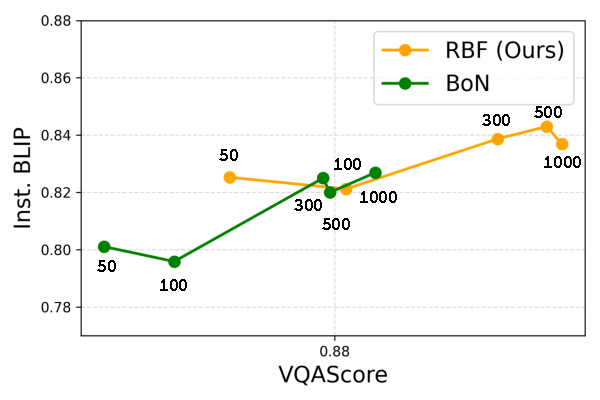
\includegraphics[width=\linewidth]{Figures/scaling/compo_nfe_scaling.pdf}
        \caption{
        \textbf{Compositional text-to-image generation scaling behavior comparison of BoN and \Ours{}.} 
        We plot the known reward (VQAScore)~\cite{Lin:2024CLIPFlanT5} against the held-out reward~\cite{Dai:2023InstructBLIP} for different numbers of function evaluations: $\{ 50, 100, 300, 500, 1,000 \}$. 
        }
        \label{fig:composition_nfe_scaling_plot}
    \end{minipage}
\end{figure*}


% \begin{figure*}[t!]
%     \centering
%     \begin{minipage}{0.48\linewidth}
%         \centering
%         {\scriptsize
%         \setlength{\tabcolsep}{0.0em}
%         \def\arraystretch{0.0}
%         \newcolumntype{Z}{>{\centering\arraybackslash}m{\linewidth}}
%         \begin{tabularx}{\linewidth}{Z}
%             \includegraphics[width=\linewidth]{Figures/scaling/Accuracy_scaling.PNG}
%         \end{tabularx}
%         }
%         \caption{\textbf{NFE scaling comparison of BoN and \Ours{}.} The x-axis has a log scale. We plot known reward (MSE)~\cite{Liu:2024GroundingDINO} against the held-out reward. The scalars on the graph indicate the number of function evaluations (NFEs).}
%         \label{fig:appendix_nfe_scaling}
%     \end{minipage}
%     \hfill
%     \begin{minipage}{0.48\linewidth}
%         \centering
%         \small
%         \setlength{\tabcolsep}{2.9pt}
%         \captionof{table}{\textbf{Quantitative results of quantity-aware image generation in NFE scaling expriment.} We use the same $100$ prompts from T2I-CompBench~\cite{Huang:2025T2ICompBench++} as in the main paper. \textsuperscript{\textdagger} denotes the given reward used in the inference-time.}
%         \label{tab:appendx_counting_nfe}
%         \newcolumntype{Z}{>{\centering\arraybackslash}m{0.01\textwidth}}
%         \newcolumntype{Y}{>{\centering\arraybackslash}m{0.1\textwidth}}
%         \newcolumntype{X}{>{\centering\arraybackslash}m{0.12\textwidth}}
%         \begin{tabular}{Z X | Y Y Y Y}
%             \toprule
%             & NFE & \scriptsize{\textbf{MSE}\textsuperscript{\textdagger}} $\downarrow$ & \scriptsize{Accuracy.} $\uparrow$ & \tiny{UniDet $\uparrow$} & \tiny{\makecell{VQA\\Score}}$\uparrow$ & \tiny{\makecell{Image\\Reward}}$\uparrow$ & \tiny{\makecell{Aesthetic\\Score $\uparrow$}} \\
%             \midrule
%             \multirow{5}{*}{\rotatebox{90}{BoN}} & 50 & 4.360 & 0.400 & 0.567 & 0.758 & 0.957 & 5.408 \\
%             & 100 & 3.280 & 0.510 & 0.602 & 0.750 & 0.976 & 5.522 \\
%             & 300 & 2.190 & 0.570 & 0.589 & 0.755 & 0.870 & 5.463 \\
%             & 500 & 1.760 & 0.580 & 0.600 & 0.756 & 0.895 & 5.420 \\
%             & 1000 & 1.340 & 0.590 & 0.605 & 0.759 & 0.900 & 5.466 \\
%             \midrule
%             \multirow{5}{*}{\rotatebox{90}{\Oursbf{}}} & 50 & 3.250 & 0.410 & 0.551 & 0.756 & 0.933 & 5.560 \\
%             & 100 & 1.860 & 0.590 & 0.596 & 0.760 & 0.951 & 5.627 \\
%             & 300 & 0.690 & 0.720 & 0.615 & 0.779 & 0.975 & 5.503 \\
%             & 500 & 0.540 & 0.800 & 0.622 & 0.769 & 0.902 & 5.581 \\
%             & 1000 & 0.290 & 0.880 & 0.634 & 0.777 & 1.013 & 5.526 \\
%             \bottomrule
%         \end{tabular}
%     \end{minipage}
% \end{figure*}
